\documentclass[a4paper]{amsart}
\usepackage{fullpage}
\setlength{\textwidth}{6.5in}
\usepackage[T1]{fontenc}
\usepackage{amsmath,amssymb,mathtools}
\usepackage{xcolor}
\usepackage{hyperref}
\usepackage{microtype,tikz,needspace}
\hypersetup{colorlinks=true,linkcolor=blue!45!black,citecolor=blue!45!black,
urlcolor=blue!45!black,pdftitle={Zeros of polyanalytic polynomials: linear bounds and explicit constructions},
pdfauthor={Antonio Lerario, Erik Lundberg, Teng Zhang}}
\newtheorem{thm}{Theorem}
\newtheorem{lem}[thm]{Lemma}
\newtheorem{prop}[thm]{Proposition}
\newtheorem{cor}[thm]{Corollary}
\newtheorem{problem}[thm]{Problem}
\newtheorem{conjecture}[thm]{Conjecture}
\theoremstyle{remark}
\newtheorem{rem}[thm]{Remark}
\newcommand{\C}{\mathbb C}
\newcommand{\R}{\mathbb R}
\newcommand{\Q}{\mathbb Q}
\newcommand{\CP}{\mathbb {CP}}
\newcommand{\eps}{\varepsilon}
\newcommand{\Nzero}{N}
\DeclareMathOperator{\Rea}{Re}
\DeclareMathOperator{\Ima}{Im}
\DeclareMathOperator{\rank}{rank}
\DeclareMathOperator{\sgn}{sgn}
\DeclareMathOperator{\sech}{sech}
\DeclareMathOperator{\csch}{csch}
\title[Zeros of polyanalytic polynomials]{Zeros of polyanalytic polynomials:\\
linear bounds and explicit constructions}
\author{Antonio Lerario}
% \address{} and \email{}: to be supplied by the author.
\author{Erik Lundberg}
% \address{} and \email{}: to be supplied by the author.
\author{Teng Zhang}
% \address{} and \email{}: to be supplied by the author.
\date{October 5, 2026}
\subjclass[2020]{Primary 30C15; Secondary 14P05, 57R40.}
\keywords{Polyanalytic polynomial, harmonic polynomial, zero counting,
Chebyshev polynomial, genus bound}
\begin{document}
\begin{abstract}
We prove that a polynomial of degree \(n\) in \(z\) and degree \(m<n\)
in \(\bar z\), with finitely many zeros, has at most
\(\min\{n^2+m^2,(4m+1)n-5m\}\) distinct zeros. The coefficient \(4m+1\)
is optimal for every fixed \(m\), and the maximal count differs from
this upper bound by at most \(4m(m-1)\).
For harmonic polynomials of analytic degree \(n\) and conjugate degree
\(m\), we construct \((m+2)n-m-\gcd(m,n)\) nondegenerate zeros.
These examples attain the known sharp bounds when \(m=1\) and \(m=n-1\).
We also determine the exact maximum in the family
\(\eps z^n+q(z)+\overline{q(z)}\), and give sparse polyanalytic
polynomials attaining the quadratic bound.
\end{abstract}
\maketitle

\section{Introduction}\label{sec:intro}

The fundamental theorem of algebra counts the zeros of a polynomial
in one complex variable by its degree. For a polynomial in \(z\) and
\(\bar z\), the zero set can instead be empty, finite, or contain a
curve. Even when it is finite, the appropriate bound depends on which
degrees are prescribed. We study the effect of fixing the degree in
the conjugate variable.

For a map \(F:\C\to\C\), write \(N(F)=\#F^{-1}(0)\).
For \(f\in\C[z,w]\), put \(F_f(z)=f(z,\bar z)\) and abbreviate
\(N(F_f)\) to \(N(f)\). All zero counts count distinct points.
A zero of a smooth map is \emph{nondegenerate} if its real
differential is invertible.
We say that \(f\) has bidegree \((n,m)\) if
\(\deg_z f=n\) and \(\deg_w f=m\), in that order. Total degree will
always be specified. Let \(M_{m,n}\) be the largest finite value of
\(N(f)\) among polynomials of bidegree \((n,m)\), where \(n>m\ge1\).
The subscript \(m\) records the conjugate degree, which we regard as
the fixed parameter.

Khavinson, Lundberg, and Perry \cite[Problem 1.9 and Proposition 1.10]{KLP24}
formulated the general valence problem for polyanalytic polynomials
and proved the bound \(n^2+m^2\) when \(f\) and
\(f^*(z,w)=\overline{f(\bar w,\bar z)}\) are coprime. Eremenko
\cite[p.~1]{Ere26} asked whether the growth is linear in \(n\) for fixed
\(m\). The finite-zero-set formulation is as follows.

\begin{problem}\label{prob:linear}
For each \(m\ge1\), do there exist constants \(A_m,B_m\) such that
\(N(f)\le A_m n+B_m\) for every polynomial of bidegree \((n,m)\),
\(n>m\), with finite zero set?
\end{problem}

Finiteness is essential: \(z^{n-m}(zw-1)^m\) vanishes on the unit
circle. Also, \(n\) in Problem~\ref{prob:linear} is not the total
degree. For example, \((z^2-a^2)\bar z-z\), with \(0<a<1\), has
bidegree \((2,1)\) and the five distinct zeros
\(0,\ \pm\sqrt{1+a^2},\ \pm i\sqrt{1-a^2}\). Thus \(n^2\) is not an
upper bound in the rectangular coefficient space.

Our first result answers Problem~\ref{prob:linear} and determines its
optimal leading constant.

\begin{thm}\label{thm:linear}
For every \(n>m\ge1\),
\begin{equation}\label{eq:mainbound}
 M_{m,n}\le U_{m,n}:=\min\{n^2+m^2,(4m+1)n-5m\}.
\end{equation}
For each fixed \(m\ge1\), one has
\(\displaystyle\lim_{n\to\infty}M_{m,n}/n=4m+1\).
\end{thm}

The estimate includes degenerate zeros and polynomials with common
factors with \(f^*\). Its proof first replaces such zeros by
nondegenerate zeros without increasing either degree. The complex
curve \(f=0\) in \(\CP^1\times\CP^1\) then gives an immersed surface
in \(\CP^2\). Resolving its double points and applying the genus
theorem of Kronheimer and Mrowka \cite{KM94} yields the linear term
in \eqref{eq:mainbound}. Eremenko's maintained problem list
\cite{EreList} records a solution of the growth question by this
reduction; the proof and the optimality assertion are given here
in full.

The lower bounds can be made uniform in both degrees. We use
\(x_+=\max\{x,0\}\) for a real number \(x\).

\Needspace{9\baselineskip}
\begin{thm}\label{thm:rectlower}
For every \(n>m\ge1\),
\begin{equation}\label{eq:uniform}
 U_{m,n}-4m(m-1)\le M_{m,n}.
\end{equation}
One has \(M_{m,n}=n^2+m^2\) when \(m<n\le2m+1\). For
\(n\ge2m+1\), there are polynomials of exact bidegree \((n,m)\)
with exactly
\begin{equation}\label{eq:lowercount}
 (4m+1)(n-m)+(3m-n)_+(3m+1-n)_+
\end{equation}
nondegenerate zeros. The constructions may be chosen with
coefficients in \(\Q(i)\).
\end{thm}

In particular, \eqref{eq:mainbound} and \eqref{eq:uniform} give
\(M_{1,n}=5n-5\). This endpoint is consistent with the theory of
rational harmonic functions developed by Khavinson and Neumann
\cite{KN06}, together with the sharp examples of Rhie \cite{Rhi03}.
For general \(m\), Theorem~\ref{thm:rectlower} leaves an additive
error depending only on \(m\); it does not determine every finite-degree
maximum.

\subsection{Harmonic polynomials}
Let \(H_{m,n}\) denote the largest zero count of
\(h(z)=p(z)+\overline{q(z)}\), where \(\deg p=n>\deg q=m\).
Subtracting a constant preserves these degrees, so this is also the
maximal valence in this class. The harmonic valence problem was
raised by Sheil-Small \cite[p.~19]{SS92} in 1992; see also Khavinson and
\'{S}wi\k{a}tek \cite{KS03}. Wilmshurst \cite{WilThesis,Wil98}
proved \(H_{m,n}\le n^2\) and constructed examples attaining this
bound for \(m=n-1\). An independent extremal construction was given
by Bshouty, Hengartner, and Suez \cite{BHS95}; Peretz and Schmid
\cite{PS97} gave an algebraic treatment of the quadratic bound.
For \(m=1\), Khavinson and \'{S}wi\k{a}tek \cite{KS03} proved the
upper bound \(3n-2\), and Geyer \cite{Gey08} proved sharpness through
holomorphic dynamics.

Wilmshurst \cite[Remark 2]{Wil98} proposed the more precise expression
\(3n-2+m(m-1)\). Lee, Lerario, and Lundberg \cite{LLL15}
disproved it and proposed linear growth for each fixed \(m\).
Further constructions were obtained by Hauenstein, Lerario,
Lundberg, and Mehta \cite{HLLM15}, Lee and Saez \cite{LS17}, and
Khavinson, Lee, and Saez \cite{KLS18}. Lundberg \cite{Lun23}
proved \(H_{m,n}\ge\lceil n\sqrt m\rceil\) by a probabilistic
argument and asked for constructions with order \(mn\) zeros.
Gao and Liu \cite{GL26} recently obtained further examples at
\(m=n-1\) using alternating analytic and anti-analytic terms.
Theorem~\ref{thm:linear} proves the fixed-\(m\) linear upper bound
in the larger polyanalytic class. The following examples give a
lower bound of order \(mn\) within the harmonic class itself.

Let \(T_j\) be the Chebyshev polynomial defined by
\(T_j(\cos\theta)=\cos(j\theta)\).

\begin{thm}\label{thm:cheb}
Let \(1\le m<n\) and \(a>2\). For all sufficiently small \(\eps>0\),
the harmonic polynomial
\begin{equation}\label{eq:chebfamily}
 h_\eps(z)=\eps T_n(z)-2\Ima T_m(z-a)
\end{equation}
has exactly \((m+2)n-m-\gcd(m,n)\) nondegenerate zeros.
\end{thm}

Here \(p(z)=\eps T_n(z)+iT_m(z-a)\) and \(q(z)=iT_m(z-a)\)
give \(h_\eps=p+\bar q\). Both degrees are exact, and rational
choices of \(a\) and \(\eps\) give coefficients in \(\Q(i)\).
Theorem~\ref{thm:cheb} implies
\begin{equation}\label{eq:harmbounds}
 (m+2)n-m-\gcd(m,n)
 \le H_{m,n}\le \min\{n^2,(4m+1)n-5m\}.
\end{equation}
The lower bound in \eqref{eq:harmbounds} is at least \(mn\),
and it recovers the sharp counts \(3n-2\) and \(n^2\) at
\(m=1\) and \(m=n-1\), respectively.

The case \(m=1\) has a particularly simple explicit form.

\begin{cor}\label{cor:explicit}
For every \(n\ge2\), the polynomial
\(p_n(z)=z-iT_n(z)/n^2\) satisfies
\(\#\{z:p_n(z)=\bar z\}=3n-2\), and every zero of
\(p_n(z)-\bar z\) is nondegenerate.
\end{cor}

We prove Corollary~\ref{cor:explicit} directly, without any
divisibility argument. The \(n\) real zeros of \(T_n\) are joined
by two nonreal zeros for each of its \(n-1\) conjugate pairs of
branches of \(\Ima T_n=0\). We also determine every transition in the zero
count of \(\eps T_n(z)-2\Ima z\), including the singular parameters.

Lundberg's question can be answered in the more restrictive family
used in his probabilistic construction. We state the question in
the form relevant to the present result.

\begin{problem}\label{prob:deterministic}
For \(1\le m<n\), choose \(\deg q=m\) and \(\eps\ne0\)
deterministically so that \(\eps z^n+q(z)+\overline{q(z)}\)
has at least \(mn\) distinct zeros.
\end{problem}

Problem~\ref{prob:deterministic} is posed by Lundberg
\cite[Section 4.2]{Lun23}. Define \(S_{m,n}\) to be the maximal
zero count in its displayed family and, with \(g=\gcd(m,n)\), put
\(\delta_{m,n}=g\) if \(m/g\) and \(n/g\) are both odd, and
\(\delta_{m,n}=0\) otherwise.

\begin{thm}\label{thm:monomial}
For every \(1\le m<n\),
\begin{equation}\label{eq:monomialmax}
 S_{m,n}=n(m+1)+\delta_{m,n}.
\end{equation}
The maximum is attained with \(\eps\in\Q_{>0}\) and
\(q\in\Q(i)[z]\), with all zeros nondegenerate.
\end{thm}

The exact value in \eqref{eq:monomialmax} concerns this particular
family. Neither it nor Theorem~\ref{thm:cheb} asserts an exact formula
for \(H_{m,n}\) at all degrees. In particular, the stronger conjecture
of Lee, Lerario, and Lundberg \cite{LLL15} that the number of
orientation-reversing zeros is at most \(m(n-1)\) is not resolved here.

\subsection{Sparse extremizers and organization}
S\`ete and Zur \cite[Remark 4.4]{SZ24} asked how many nonzero
coefficients are necessary for a polynomial of total degree \(d\)
to have \(d^2\) zeros, and proposed the following conjecture.

\begin{conjecture}\label{conj:sparse}
A polyanalytic polynomial of total degree \(d\) with \(d^2\)
distinct zeros has at least \(d\) nonzero coefficients.
\end{conjecture}

The radial constructions used for Theorem~\ref{thm:rectlower}
also give counterexamples to Conjecture~\ref{conj:sparse}.

\begin{thm}\label{thm:sparse}
For every \(d\ge2\), there is a polynomial of total degree \(d\)
with coefficients in \(\Q\), exactly \(\lceil d/2\rceil+1\)
nonzero monomials, and \(d^2\) nondegenerate zeros.
The least possible number of monomials in total degree four
is three, attained by
\begin{equation}\label{eq:quartic}
 z^4+z\bar z^2-\tfrac18\bar z.
\end{equation}
\end{thm}

Section~\ref{sec:cheb} gives the harmonic Chebyshev construction,
beginning with the explicit \(m=1\) example.
Section~\ref{sec:regular} proves the perturbation and intersection
lemmas, and Section~\ref{sec:genus} proves the linear upper bound.
Section~\ref{sec:radial} supplies the radial constructions and proves
Theorems~\ref{thm:rectlower} and~\ref{thm:sparse}.
Section~\ref{sec:monomial} proves the exact restricted harmonic
maximum. Section~\ref{sec:questions} records the remaining questions.
All proofs in the paper are independent of numerical certification.
The supplementary repository \cite{Supplement} contains reproducible
checks, figures, a proof audit, and the original research archive.

\section{Chebyshev polynomials and harmonic zeros}\label{sec:cheb}

\subsection{The real-level curves}
The identity \(T_n(\cos\zeta)=\cos(n\zeta)\) holds for complex
\(\zeta\), by the polynomial recurrence for \(T_n\).
Every point of the upper half-plane has a unique representation
\begin{equation}\label{eq:coordinates}
 z=\cos(\theta-it)=\cos\theta\cosh t+i\sin\theta\sinh t,
 \qquad 0<\theta<\pi,\quad t>0.
\end{equation}
Indeed, of the two solutions of \(\xi+\xi^{-1}=2z\), exactly one
has modulus greater than one. Its imaginary part is positive,
and writing it as \(e^{t+i\theta}\) gives \eqref{eq:coordinates}.
The differential is nonsingular: its determinant is
\(-(\sin^2\theta+\sinh^2t)<0\).
Since \(\Ima T_n(z)=\sin(n\theta)\sinh(nt)\), the nonreal upper
branches of the real-level set are
\begin{equation}\label{eq:branches}
 z_j(t)=\cos\theta_j\cosh t+i\sin\theta_j\sinh t,\qquad
 \theta_j=\frac{j\pi}{n},\quad 1\le j<n,\quad t>0.
\end{equation}
The remaining branches are their complex conjugates and the real
axis. On the \(j\)-th branch, \(T_n(z_j(t))=(-1)^j\cosh(nt)\).

\subsection{A complete count when the conjugate degree is one}
For \(m=1\), the real translation in \eqref{eq:chebfamily} disappears:
\(\Ima T_1(z-a)=\Ima z\). Put
\(\phi_n(t)=\sinh t/\cosh(nt)\) for \(t>0\).
Its logarithmic derivative is
\(\coth t-n\tanh(nt)\), whose derivative is
\(-\csch^2t-n^2\sech^2(nt)<0\).
The logarithmic derivative tends to \(+\infty\) at zero and to
\(1-n<0\) at infinity. Thus there is a unique \(t_n>0\) satisfying
\begin{equation}\label{eq:tn}
 \coth t_n=n\tanh(nt_n).
\end{equation}
The function \(\phi_n\) increases on \((0,t_n)\), decreases on
\((t_n,\infty)\), and tends to zero at both ends.
Define \(b_{n,j}=2\sin(j\pi/n)\phi_n(t_n)\), for \(1\le j<n\).

\begin{prop}\label{prop:allparameters}
For \(n\ge2\) and \(\eps>0\), let
\(f_{n,\eps}(z)=\eps T_n(z)-2\Ima z\). Then
\begin{equation}\label{eq:parametercount}
 N(f_{n,\eps})=
 n+2\#\{1\le j<n:\eps<b_{n,j}\}
   +\#\{1\le j<n:\eps=b_{n,j}\}.
\end{equation}
Every zero is nondegenerate unless \(\eps=b_{n,j}\) for some \(j\).
At such a parameter there is exactly one degenerate zero for
each index \(j\) with \(\eps=b_{n,j}\).
\end{prop}

\begin{proof}
On the real axis, \(f_{n,\eps}\) has the \(n\) simple zeros of \(T_n\).
At each such point \(x\), its Jacobian is \(\eps^2T_n'(x)^2>0\).
On the upper branch \(z_j(t)\), its real part vanishes precisely when
\(\eps(-1)^j=2\sin\theta_j\phi_n(t)\).
On the reflected lower branch, the corresponding equation is
\(\eps(-1)^j=-2\sin\theta_j\phi_n(t)\).
Only the upper branch is possible for even \(j\), and only the lower
branch for odd \(j\). On the selected branch, the equation reduces to
\begin{equation}\label{eq:onecurve}
 \eps=2\sin\theta_j\,\phi_n(t).
\end{equation}
The monotonicity established before \eqref{eq:tn} gives two, one,
or no solutions according as \(\eps<b_{n,j}\),
\(\eps=b_{n,j}\), or \(\eps>b_{n,j}\). This proves
\eqref{eq:parametercount}.

The derivative of the imaginary part in the transverse
\(\theta\)-direction is, up to sign,
\(\eps n(-1)^j\sinh(nt)\ne0\). Along the selected branch, the
derivative of the real part at a zero is a nonzero factor times
\(\phi_n'(t)\). In the regular coordinates \eqref{eq:coordinates},
these derivatives prove nondegeneracy except at \(t=t_n\).
At \(t_n\), the differential has rank one. Moreover,
\(\phi_n''(t_n)<0\), because the logarithmic derivative is strictly
decreasing. The two roots of \eqref{eq:onecurve} therefore meet in a
quadratic tangency, and the stated degenerate zeros are the only ones.
\end{proof}

We now prove the explicit assertion of Corollary~\ref{cor:explicit}.
The minimum of the \(b_{n,j}\) is \(b_{n,1}\), and
\begin{equation}\label{eq:threshold}
 b_{n,1}\ge
 \frac{2\sin(\pi/n)\sinh(1/n)}{\cosh1}
 \ge \frac{4}{n^2\cosh1}>\frac1{n^2}.
\end{equation}
Here \(\sin(\pi/n)\ge2/n\), \(\sinh(1/n)\ge1/n\), and
\(\cosh1<4\). Equations~\eqref{eq:parametercount} and
\eqref{eq:threshold} show that \(f_{n,1/n^2}\) has \(n+2(n-1)\)
nondegenerate zeros. Finally,
\(-if_{n,1/n^2}=z-iT_n(z)/n^2-\bar z=p_n(z)-\bar z\).
Multiplication by \(-i\) preserves zeros and nondegeneracy, completing
the proof.

The location of the additional roots explains why the linearity
of \(T_1\) does not reduce the count. On every selected branch,
one solution of \eqref{eq:onecurve} approaches \(t=0\), and the
other approaches infinity as \(\eps\) decreases to zero.
Thus there are \(n-1\) roots near the real critical points of \(T_n\)
and \(n-1\) roots escaping to infinity, in addition to its \(n\)
real roots.

Figure~\ref{fig:chebyshev} illustrates the count when \(n=5\).

\begin{figure}[htbp]
\centering
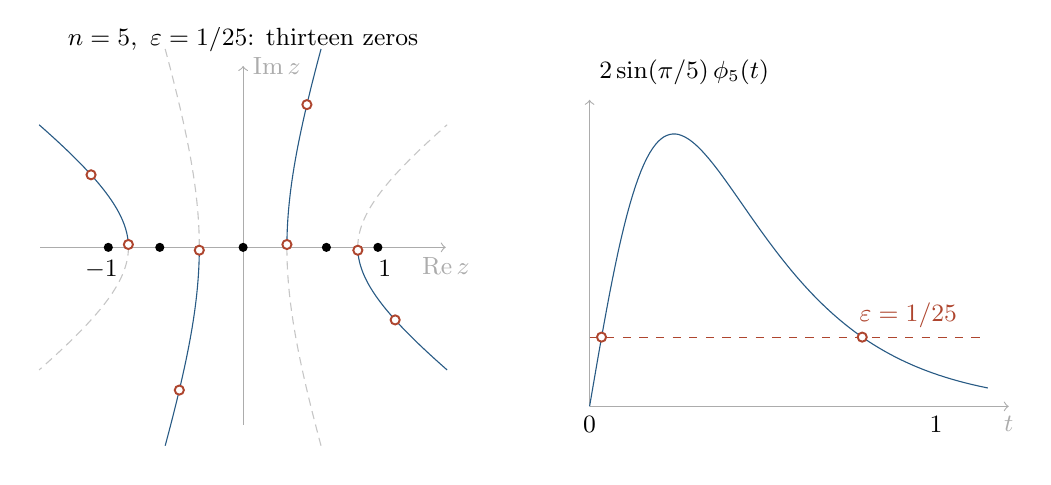
\begin{tikzpicture}[font=\small]
\definecolor{curveblue}{RGB}{40,90,132}
\definecolor{rootred}{RGB}{174,69,46}
\begin{scope}[x=1.8cm,y=1.8cm]
\clip (-1.52,-1.48) rectangle (1.64,1.55);
\draw[gray!65,->] (-1.43,0)--(1.43,0) node[below] {\(\Rea z\)};
\draw[gray!65,->] (0,-1.25)--(0,1.28) node[right] {\(\Ima z\)};
\node at (0,1.47) {\(n=5,\ \eps=1/25\): thirteen zeros};
\draw[curveblue,thin,domain=0:1.18,samples=90,variable=\t] plot ({cos(36.0)*(exp(\t)+exp(-\t))/2},{-1*sin(36.0)*(exp(\t)-exp(-\t))/2});
\draw[gray!45,densely dashed,thin,domain=0:1.18,samples=90,variable=\t] plot ({cos(36.0)*(exp(\t)+exp(-\t))/2},{1*sin(36.0)*(exp(\t)-exp(-\t))/2});
\draw[curveblue,thin,domain=0:1.18,samples=90,variable=\t] plot ({cos(72.0)*(exp(\t)+exp(-\t))/2},{1*sin(72.0)*(exp(\t)-exp(-\t))/2});
\draw[gray!45,densely dashed,thin,domain=0:1.18,samples=90,variable=\t] plot ({cos(72.0)*(exp(\t)+exp(-\t))/2},{-1*sin(72.0)*(exp(\t)-exp(-\t))/2});
\draw[curveblue,thin,domain=0:1.18,samples=90,variable=\t] plot ({cos(108.0)*(exp(\t)+exp(-\t))/2},{-1*sin(108.0)*(exp(\t)-exp(-\t))/2});
\draw[gray!45,densely dashed,thin,domain=0:1.18,samples=90,variable=\t] plot ({cos(108.0)*(exp(\t)+exp(-\t))/2},{1*sin(108.0)*(exp(\t)-exp(-\t))/2});
\draw[curveblue,thin,domain=0:1.18,samples=90,variable=\t] plot ({cos(144.0)*(exp(\t)+exp(-\t))/2},{1*sin(144.0)*(exp(\t)-exp(-\t))/2});
\draw[gray!45,densely dashed,thin,domain=0:1.18,samples=90,variable=\t] plot ({cos(144.0)*(exp(\t)+exp(-\t))/2},{-1*sin(144.0)*(exp(\t)-exp(-\t))/2});
\fill[black] (0.951056516,0.000000000) circle (1.65pt);
\fill[black] (0.587785252,0.000000000) circle (1.65pt);
\fill[black] (0.000000000,0.000000000) circle (1.65pt);
\fill[black] (-0.587785252,0.000000000) circle (1.65pt);
\fill[black] (-0.951056516,0.000000000) circle (1.65pt);
\fill[draw=rootred,fill=white,line width=.7pt] (0.809499276,-0.020298778) circle (1.65pt);
\fill[draw=rootred,fill=white,line width=.7pt] (1.072767415,-0.511849819) circle (1.65pt);
\fill[draw=rootred,fill=white,line width=.7pt] (0.309086081,0.020111885) circle (1.65pt);
\fill[draw=rootred,fill=white,line width=.7pt] (0.450074280,1.007091018) circle (1.65pt);
\fill[draw=rootred,fill=white,line width=.7pt] (-0.309086081,-0.020111885) circle (1.65pt);
\fill[draw=rootred,fill=white,line width=.7pt] (-0.450074280,-1.007091018) circle (1.65pt);
\fill[draw=rootred,fill=white,line width=.7pt] (-0.809499276,0.020298778) circle (1.65pt);
\fill[draw=rootred,fill=white,line width=.7pt] (-1.072767415,0.511849819) circle (1.65pt);
\node[below] at (-1,-.025) {\(-1\)};
\node[below] at (1,-.025) {\(1\)};
\end{scope}
\begin{scope}[shift={(4.4cm,-2.02cm)},x=4.4cm,y=22cm]
\draw[gray!65,->] (0,0)--(1.21,0) node[below] {\(t\)};
\draw[gray!65,->] (0,0)--(0,.177);
\node[anchor=south west] at (0,.18) {\(2\sin(\pi/5)\,\phi_5(t)\)};
\draw[curveblue,domain=0:1.15,samples=140,variable=\t] plot (\t,{2*sin(36)*(exp(\t)-exp(-\t))/(exp(5*\t)+exp(-5*\t))});
\draw[rootred,dashed] (0,.04)--(1.15,.04);
\node[rootred,above] at (.92,.04) {\(\eps=1/25\)};
\fill[draw=rootred,fill=white,line width=.7pt] (0.034527483,.04) circle (1.65pt);
\fill[draw=rootred,fill=white,line width=.7pt] (0.787012851,.04) circle (1.65pt);
\node[below] at (0,0) {\(0\)};
\node[below] at (1,0) {\(1\)};
\end{scope}
\end{tikzpicture}
\caption{The degree-five example. Filled dots are the five real zeros;
open circles are the eight nonreal zeros. Solid curves are the selected
branches of \(\Ima T_5=0\); their conjugates are dashed.
The right panel shows the two intersections that occur on each
selected branch, here for \(j=1\) and \(j=4\).}
\label{fig:chebyshev}
\end{figure}


\subsection{Intersections of translated branches}
We next prove Theorem~\ref{thm:cheb}. At height \(y>0\), the real
coordinate of a branch with angle \(\theta\) is
\(X_\theta(y)=\cot\theta\sqrt{y^2+\sin^2\theta}\).
The upper branches of \(\Ima T_m(z-a)=0\) have real coordinates
\(a+X_{\varphi_\ell}(y)\), where
\(\varphi_\ell=\ell\pi/m\), \(1\le\ell<m\).

\begin{lem}\label{lem:crossing}
Let \(a>2\) and \(0<\theta,\varphi<\pi\).
The curves \(x=X_\theta(y)\) and \(x=a+X_\varphi(y)\),
\(y>0\), have exactly one intersection if \(\theta<\varphi\),
and no intersection otherwise. Every intersection is transverse.
\end{lem}

\begin{proof}
For fixed \(y\), \(X_\theta(y)\) is strictly decreasing in \(\theta\):
write it as
\(\cos\theta\sqrt{1+y^2/\sin^2\theta}\) and differentiate.
Thus \(\theta\ge\varphi\) gives no intersection.
If \(\theta<\varphi\), the function
\(X_\theta(y)-X_\varphi(y)\) starts at
\(\cos\theta-\cos\varphi\in(0,2)\) and tends to infinity.
It is strictly increasing for \(y>0\). To see this, note that
\(X_\theta'(y)=y\cot\theta/\sqrt{y^2+\sin^2\theta}\), and
\[
 \frac{\partial}{\partial\theta}
 \frac{\cot\theta}{\sqrt{y^2+\sin^2\theta}}
 =
 -\frac{1}{\sin^2\theta\sqrt{y^2+\sin^2\theta}}
 -\frac{\cos^2\theta}{(y^2+\sin^2\theta)^{3/2}}<0.
\]
The equation \(X_\theta(y)-X_\varphi(y)=a\) has exactly one
solution, at which its derivative is positive.
\end{proof}

For the branch \(z_j\) in \eqref{eq:branches}, let
\(k_j=\#\{1\le\ell<m:j/n<\ell/m\}\). Lemma~\ref{lem:crossing}
says that these are exactly the simple zeros of
\(\Ima T_m(z_j(t)-a)\) for \(t>0\). There are \(g-1\) equality
pairs \(j/n=\ell/m\), where \(g=\gcd(m,n)\); reflection
\((j,\ell)\mapsto(n-j,m-\ell)\) interchanges the strict inequalities.
Hence
\begin{equation}\label{eq:crossingcount}
 \sum_{j=1}^{n-1}k_j=
 \frac{(n-1)(m-1)-(g-1)}2.
\end{equation}

\subsection{Counting small levels}
Put \(r(z)=T_m(z-a)\) and
\(A_j(t)=2\Ima r(z_j(t))/\cosh(nt)\).
The upper branch requires \(A_j(t)=\eps(-1)^j\), and the lower
branch requires \(A_j(t)=-\eps(-1)^j\).
Together these are the two levels \(A_j(t)=\pm\eps\).

At the finite endpoint,
\(A_j(t)=2r'(\cos\theta_j)\sin\theta_j\,t+O(t^2)\).
Its linear coefficient is nonzero: the roots of \(T_m'\) lie in
\((-1,1)\), whereas \(\cos\theta_j-a<-1\); for \(m=1\) the
derivative is one. At the other end, expand
\(r=\sum_{k=0}^m c_kT_k\), with real coefficients.
Then
\(\Ima r(z_j(t))=\sum_{k=1}^m c_k\sin(k\theta_j)\sinh(kt)\).
This sum is not identically zero, as its derivative at zero is
nonzero. Let \(\kappa_j\) be the largest index for which
\(c_k\sin(k\theta_j)\ne0\). Since \(1\le\kappa_j\le m<n\),
there is a nonzero real constant \(C_j\) such that
\begin{equation}\label{eq:endbehavior}
 \begin{split}
 A_j(t)&=C_j e^{-(n-\kappa_j)t}(1+o(1)),\\
 A_j'(t)&=-(n-\kappa_j)C_j e^{-(n-\kappa_j)t}(1+o(1)).
 \end{split}
\end{equation}
These estimates follow by differentiating the finite exponential
sums, so the derivative estimate is justified separately.
In particular, \(A_j\) is eventually strictly monotone and tends
to zero. The index \(\kappa_j\) is needed when
\(\sin(m\theta_j)=0\).

We now complete the proof of Theorem~\ref{thm:cheb}.

\begin{proof}
\emph{Step 1: counting each pair of branches.}
Choose disjoint small intervals around the \(k_j\) simple interior
zeros of \(A_j\), an initial interval on which \(A_j'\ne0\),
and a terminal interval on which \eqref{eq:endbehavior} applies.
Each interior interval contains one solution to each level
\(A_j=\eps\) and \(A_j=-\eps\), for all sufficiently small
\(\eps>0\). The initial and terminal intervals each contain
exactly one solution to one of the two levels.
The remaining set is compact and contains no zero of \(A_j\);
its positive minimum of \(|A_j|\) excludes any further solution.
Thus the pair contributes exactly \(2k_j+2\) simple solutions.

\emph{Step 2: completeness and regularity.}
On the real axis the zeros are exactly the \(n\) simple roots of
\(T_n\). Their Jacobians equal
\(|\eps T_n'(x)+ir'(x)|^2-|ir'(x)|^2
=\eps^2T_n'(x)^2>0\).
At a nonreal zero, the real derivative along its branch is a
nonzero factor times \(A_j'(t)\), and the imaginary derivative
transverse to the branch is, up to sign,
\(\eps n(-1)^j\sinh(nt)\ne0\).
The coordinates \eqref{eq:coordinates} are regular, so the planar
Jacobian is nonzero. A common sufficiently small parameter works
for all \(n-1\) pairs.
The complete description of the real-level set after
\eqref{eq:branches}, followed by \eqref{eq:crossingcount}, gives
\[
 N(h_\eps)=n+\sum_{j=1}^{n-1}(2k_j+2)
          =(m+2)n-m-g.
\]
This proves the theorem.
\end{proof}

The examples also give a uniform collection of counterexamples to
the original Wilmshurst conjecture.

\begin{cor}\label{cor:wilm}
For \(2\le m\le n-2\), with \((m,n)\ne(2,4)\), there is a
harmonic polynomial of degrees \((n,m)\) with more than
\(3n-2+m(m-1)\) distinct zeros.
\end{cor}

\begin{proof}
Subtracting the proposed count from Theorem~\ref{thm:cheb} gives
\((m-1)(n-m-1)+1-\gcd(m,n)\).
If \(n-m\ge3\), this is at least
\((m-1)(n-m-2)>0\).
If \(n-m=2\), it equals \(m-\gcd(m,2)\), which is positive
except for \(m=2\).
\end{proof}

\section{Perturbation and intersection bounds}\label{sec:regular}

For \(f\in\C[z,w]\), its real Jacobian on \(w=\bar z\) is
\begin{equation}\label{eq:jacobian}
 J_f(z)=|f_z(z,\bar z)|^2-|f_w(z,\bar z)|^2.
\end{equation}
A zero is \emph{nondegenerate} if \(J_f\ne0\).
The real differential has rank zero exactly when \(f_z=f_w=0\).
Nondegenerate zeros persist uniquely under sufficiently small
coefficient perturbations. A constant perturbation need not
preserve all isolated zeros, so a different perturbation is needed.

We use the following standard form of parametric transversality.
All manifolds in its statement are finite dimensional and
second countable.

\begin{lem}[{\cite[Chapter 3, Section 2]{Hir76}}]\label{lem:transversality}
Let \(B,Y,Z\) be smooth manifolds, let \(W\subset Z\) be a
smooth submanifold, and let \(\mathcal F:B\times Y\to Z\)
be a smooth map transverse to \(W\).
For a residual set of \(b\in B\), the map
\(\mathcal F_b:Y\to Z\) is transverse to \(W\).
\end{lem}

The local observation below explains the use of opposite parameters.

\begin{lem}\label{lem:rankone}
Let \(F:(\R^2,0)\to(\R^2,0)\) be real analytic with an
isolated zero and \(\rank DF(0)=1\).
Let \(G\) be real analytic near zero, with
\(G(0)\notin\operatorname{im}DF(0)\).
For every sufficiently small \(t>0\), the total number of
nondegenerate zeros of \(F+tG\) and \(F-tG\) in a fixed
neighborhood of zero is at least two.
The assertion is uniform when \(G\) varies in a sufficiently
small finite-dimensional neighborhood.
\end{lem}

\begin{proof}
Real analytic source coordinates and an invertible real linear
target change put \(F\) in the form \(F(x,y)=(x,g(x,y))\), with
\(Dg(0)=0\). Isolation implies
\(g(0,y)=cy^\ell+O(y^{\ell+1})\), where \(c\ne0\) and \(\ell\ge2\).
Write \(G=(G_1,G_2)\) in these coordinates and put
\(\beta=G_2(0)\ne0\).
The first equation of \(F\pm tG=0\) has a unique solution
\(x=X_\pm(y,t)=O(t)\). Substitute \(y=t^{1/\ell}u\) into the
second equation and divide by \(t\). The resulting functions
converge in \(C^1\), on bounded \(u\)-intervals, to
\(cu^\ell\pm\beta\). Indeed, every mixed term of \(g\) contains
\(x\) and has order at least two; after substitution its
contribution, and its \(u\)-derivative, tend to zero.
The same holds for the nonconstant terms of \(G_2\).
For odd \(\ell\), each limiting equation has one simple real
root. For even \(\ell\), one has two simple real roots.
The implicit function theorem preserves these roots and the
nonvanishing two-dimensional Jacobian. The argument is uniform
under the stated variation of \(G\).
\end{proof}

\begin{lem}\label{lem:regularization}
Let \(f\in\C[z,w]\) have finitely many zeros on \(w=\bar z\).
Every coefficient neighborhood of \(f\) contains a polynomial
\(\widetilde f\) such that
\(\deg_z\widetilde f\le\deg_z f\),
\(\deg_w\widetilde f\le\deg_w f\),
and \(N(\widetilde f)\ge N(f)\), with all zeros nondegenerate.
The perturbation may be taken in any complex linear coefficient
space containing \(f\) and stable under \(\partial_z,\partial_w\).
\end{lem}

\begin{proof}
\emph{Step 1: generic perturbations away from rank-zero zeros.}
Set \(S_f=\{z:f=f_z=f_w=0\text{ at }(z,\bar z)\}\), which is
finite, and let \(f_\xi=f+\xi_1f_z+\xi_2f_w\), with
\(\xi=(\xi_1,\xi_2)\in\C^2\).
At a zero of \(f_\xi\) outside \(S_f\), at least one of
\(f_z,f_w\) is nonzero. The differential with respect to \(\xi\)
is therefore onto \(\C\). Lemma~\ref{lem:transversality}
shows that, for a residual set of \(\xi\), all zeros outside
\(S_f\) are nondegenerate. We impose this condition on both
\(\xi\) and \(-\xi\). The zero sets are finite: if a real
algebraic zero set with singularities confined to a finite set
were infinite, its complement of that finite set would be an
infinite discrete semialgebraic set, which is impossible.

\emph{Step 2: a choice of sign preserving the count.}
At every rank-one zero, the map
\((a,b)\mapsto af_z+bf_w\) is onto \(\C\).
Choose \((a,b)\in\C^2\) so its value avoids the one-dimensional
real image of \(dF_f\) at each such zero.
Only finitely many proper real linear subspaces are excluded.
Lemma~\ref{lem:rankone}, in disjoint neighborhoods of the
rank-one zeros, gives at least two nondegenerate zeros in total
for the two signs. Rank-two zeros persist for both signs,
and the points of \(S_f\) remain zeros for both signs.
Uniformity in Lemma~\ref{lem:rankone} gives an open cone of
small parameters with these properties. We may choose \(\xi\)
in that cone satisfying Step~1; then
\begin{equation}\label{eq:opposite}
 N(f_\xi)+N(f_{-\xi})\ge2N(f).
\end{equation}

\emph{Step 3: termination.}
At each point of \(S_f\), let \(H_k\) be the first nonzero
homogeneous term of the complex Taylor expansion of \(f\);
here \(k\ge2\). Require also
\(a(H_k)_z+b(H_k)_w\not\equiv0\).
This excludes finitely many further proper complex linear
subspaces. For every nonzero parameter in a suitable smaller
cone, the vanishing order of \(f_{\pm\xi}\) at each of these
points is \(k-1\).
Choose a sign in \eqref{eq:opposite} with at least \(N(f)\)
zeros, and repeat. After the first step, every degenerate
zero belongs to the original finite set \(S_f\).
At any point that remains rank zero the vanishing order
strictly decreases. Once it reaches one, that point has rank
one or two, and a further step removes any remaining degeneracy.
The procedure therefore terminates.
Successively smaller perturbations keep the final polynomial
in the prescribed neighborhood. Derivatives increase neither
degree, and every operation stays in the indicated coefficient
space.
\end{proof}

The argument has reduced the upper-bound problem to generic
polynomials. Let \(X=\CP^1_z\times\CP^1_w\), with involution
\(\tau(z,w)=(\bar w,\bar z)\) and fixed sphere \(L\).
An affine polynomial with \(\deg_z f\le n,\deg_w f\le m\)
is a section of \(\mathcal O_X(n,m)\).

\begin{lem}\label{lem:generic}
For \(n,m\ge1\), a dense set of sections of
\(\mathcal O_X(n,m)\) have a smooth connected zero curve \(C\)
which avoids \((\infty,\infty)\) and is transverse both to
\(L\) and to \(\tau C\).
\end{lem}

\begin{proof}
The complete linear system separates first jets, and separates
the values at any two distinct points. Its evaluation map is
a submersion, so Lemma~\ref{lem:transversality} gives smoothness
and transversality to \(L\).
Off \(L\), independent evaluation at \(x,\tau x\) gives
transversality of \(C\) and \(\tau C\).
At a fixed point, failure of this transversality would make
the complex tangent line \(T_xC\) invariant under \(d\tau_x\).
An antilinear involution on a complex line has a nonzero fixed
vector; this would contradict \(T_xC\cap T_xL=\{0\}\).
Avoiding \((\infty,\infty)\) excludes the hyperplane on which
the coefficient of \(z^nw^m\) vanishes.

A disconnected smooth divisor has disjoint irreducible
components. If two components have bidegrees
\((n_i,m_i)\) and \((n_j,m_j)\), their intersection number is
\(n_i m_j+m_i n_j\). All these integers are nonnegative.
Pairwise disjointness would force all components into the
same ruling, contrary to \(n,m>0\). Hence \(C\) is connected.
\end{proof}

We will also use the standard genus and intersection formulas.

\begin{lem}[{\cite[Chapter V, Proposition 1.5]{Har77}}]\label{lem:adjunction}
A smooth connected curve of bidegree \((n,m)\) in
\(\CP^1\times\CP^1\) has genus \((n-1)(m-1)\).
Two curves of bidegrees \((n_1,m_1)\) and \((n_2,m_2)\),
without a common component, have intersection number
\(n_1m_2+m_1n_2\).
\end{lem}

The intersection formula also underlies the coprime bound of
Khavinson, Lundberg, and Perry \cite[Proposition 1.10]{KLP24}.
Together, Lemmas~\ref{lem:regularization}--\ref{lem:adjunction}
give \(N(f)\le n^2+m^2\) whenever \(N(f)<\infty\):
after regularization, a sufficiently small perturbation
satisfying Lemma~\ref{lem:generic} preserves all displayed
zeros, and its curves \(C,\tau C\) meet in \(n^2+m^2\) points.
This proves the quadratic term of \eqref{eq:mainbound} without
a common-factor assumption.

For later constructions, the following total-degree version
also proves finiteness and detects nondegeneracy at equality.

\begin{lem}\label{lem:pure}
If \(f(z,w)=cz^d+q(z,w)\), with \(c\ne0\) and
\(\deg_{\rm tot}q<d\), then \(N(f)\le d^2\).
If \(f\) has \(d^2\) distinct zeros, all are nondegenerate.
\end{lem}

\begin{proof}
In a graded monomial order the leading monomials of \(f\)
and \(f^*\) are \(z^d,w^d\), after normalization.
They are coprime, so these two polynomials form a
Gr\"obner basis. The quotient has basis
\(\{z^iw^j:0\le i,j<d\}\) and length \(d^2\).
Every real-slice zero is an intersection of \(f,f^*\).
If there are \(d^2\) distinct such points, each local
intersection has length one. Its Jacobian determinant is
the nonzero number in \eqref{eq:jacobian}.
\end{proof}

\section{The genus bound}\label{sec:genus}

The topological input is the Thom genus theorem.

\begin{lem}[{\cite[Theorem 1]{KM94}}]\label{lem:thom}
Let \(\Sigma\) be a smooth closed connected oriented surface
embedded in \(\CP^2\), representing
\(d[\CP^1]\) with \(d\ge1\).
Then \(g(\Sigma)\ge(d-1)(d-2)/2\).
\end{lem}

By Lemmas~\ref{lem:regularization} and~\ref{lem:generic},
it suffices to consider a smooth connected curve
\(C\subset X\) of bidegree \((n,m)\), avoiding
\((\infty,\infty)\) and transverse to \(L,\tau C\).
Let \(N=\#(C\cap L)\).
The symmetric-product map
\begin{equation}\label{eq:quotient}
 \Phi:X\longrightarrow\operatorname{Sym}^2(\CP^1)\simeq\CP^2,
 \qquad (z,w)\longmapsto\{z,\bar w\}
\end{equation}
has fibers equal to the \(\tau\)-orbits. In homogeneous
coordinates it is
\([z_0:z_1],[w_0:w_1]\mapsto
[z_0\bar w_0:z_1\bar w_0+z_0\bar w_1:z_1\bar w_1]\).

\begin{lem}\label{lem:immersion}
The restriction \(\Phi|_C\) is an immersion with exactly
\((n^2+m^2-N)/2\) transverse positive double points
and no other multiple points.
\end{lem}

\begin{proof}
Away from \(L\), the map is a local diffeomorphism.
Near \(L\), put \(u=(z+\bar w)/2,\ v=(z-\bar w)/2\);
in suitable target coordinates, \(\Phi(u,v)=(u,v^2)\).
If \(J\) is the complex structure of \(X\), then
\(\ker d\Phi=J(TL)\) along \(L\).
The complex line \(TC\) is transverse to \(TL\), hence also
to \(J(TL)\). Thus \(\Phi|_C\) is immersive there.

Distinct points of \(C\) have the same image exactly when
they are \(x,\tau x\), with \(x\in(C\cap\tau C)\setminus L\).
The two branches are transverse, and no fiber has more
than two points. Lemma~\ref{lem:adjunction} gives
\(\#(C\cap\tau C)=n^2+m^2\); removing its \(N\) fixed
points and pairing the rest proves the count.
For the sign, transport the second branch to \(x\) by
\(\tau\). This reverses its complex orientation,
while \(\Phi\) reverses the ambient four-dimensional
orientation off \(L\): it is the holomorphic symmetric-product
map composed with conjugation in one factor.
The two reversals cancel, leaving
the positive intersection sign of two complex curves.
\end{proof}

We now prove the upper bound in Theorem~\ref{thm:linear}.

\begin{proof}
The quadratic bound was proved after Lemma~\ref{lem:adjunction}.
For the linear bound, resolve every double point of
Lemma~\ref{lem:immersion} by the oriented local smoothing
of two transverse complex coordinate disks. Each smoothing
replaces two disks by an annulus, preserves the homology
class, and adds one to the genus.
This gives an embedded connected oriented surface
\(\Sigma\subset\CP^2\) with
\begin{equation}\label{eq:surfacegenus}
 g(\Sigma)=(n-1)(m-1)+\frac{n^2+m^2-N}{2}.
\end{equation}
Let \(\alpha,\beta\) be the positive degree-two cohomology
generators of the two factors of \(X\), and \(H\) the
hyperplane class of \(\CP^2\).
Restriction of \eqref{eq:quotient} to the factors gives
\(\Phi^*H=\alpha-\beta\).
Since \(C\) has divisor class \(n\alpha+m\beta\), its image
has degree \(m-n\). Reverse the orientation of \(\Sigma\)
to obtain degree \(d=n-m>0\).
Lemma~\ref{lem:thom} and \eqref{eq:surfacegenus} imply
\[
 (n-1)(m-1)+\frac{n^2+m^2-N}{2}
 \ge\frac{(n-m-1)(n-m-2)}2.
\]
Rearranging gives \(N\le(4m+1)n-5m\).
The initial perturbations did not decrease the zero count,
so the same estimate holds for the original polynomial.
\end{proof}

Every value used to define \(M_{m,n}\) is an integer bounded
by \eqref{eq:mainbound}, and the class is nonempty, for
example \(z^nw^m+1\). Hence the maximum exists.
Lemma~\ref{lem:regularization}, followed by
Lemma~\ref{lem:generic}, shows that it is attained with all
zeros nondegenerate and a nonzero \(z^nw^m\) coefficient.
For such a polynomial, the mapping degree at infinity is
\(n-m\), so its positive and negative Jacobian counts
satisfy \(N_+-N_-=n-m\).
In particular, \(M_{m,n}\equiv n-m\pmod2\).

\section{Radial constructions and sharpness}\label{sec:radial}

\subsection{Real roots from separated coefficients}
Our constructions use an elementary coefficient-dominance
argument related to sign-independent real-rootedness.
The latter was studied by Passare, Rojas, and Shapiro
\cite{PRS11} and by Forsg{\aa}rd, Novikov, and Shapiro
\cite[Proposition 1]{FNS17}. We give the short form needed
here, including gaps in the exponents.

For a list of nonzero real numbers, let \(V\) be its number
of sign changes.

\begin{lem}\label{lem:dominance}
Let \(0\le e_0<\cdots<e_s\) be integers and
\(c_0,\ldots,c_s\) nonzero real numbers.
If \(0<\rho_0<\cdots<\rho_s\) satisfy
\[
 |c_i|\rho_i^{e_i}>
 \sum_{j\ne i}|c_j|\rho_i^{e_j}\qquad(0\le i\le s),
\]
then \(\sum_{i=0}^s c_i r^{e_i}\) has
\(V(c_0,\ldots,c_s)\) positive roots and
\(V((-1)^{e_0}c_0,\ldots,(-1)^{e_s}c_s)\) negative roots.
All nonzero real roots are simple.
\end{lem}

\begin{proof}
At \(\rho_i\) the polynomial has sign \(\sgn c_i\).
The intermediate value theorem gives a different positive
root for each sign change. Descartes' rule bounds the
positive roots, counted with multiplicity, by the same
number. Equality follows, and every root is simple.
Apply this argument to the polynomial at \(-r\) for the
negative roots.
\end{proof}

One choice of scales works for many polynomials at once.
If \(0<\mu\le|b_i|\le B\), set \(c_i=b_it^{e_i^2}\)
and \(\rho_i=t^{-2e_i}\), where \(0<t<1\). Then
\begin{equation}\label{eq:dominanceidentity}
 t^{e_i^2}\sum_{j=0}^s c_j\rho_i^{e_j}
 =b_i+\sum_{j\ne i}b_jt^{(e_j-e_i)^2}.
\end{equation}
The remainder in \eqref{eq:dominanceidentity} has absolute
value at most \(sBt\); thus \(sBt<\mu\) is sufficient.

\begin{lem}\label{lem:radial}
Let \(a,b\ge0\) and \(k>2b\) be integers.
Among maps
\[
 F(z)=B(|z|^2)+z^kA(|z|^2),\qquad
 \deg A=a,\quad\deg B=b,\quad B(0)\ne0,
\]
with finite zero set, the maximal zero count is
\(k(2a+2b+1)\).
It is attained with \(A,B\in\Q[t]\), with all zeros
nondegenerate and \(A,B\) having no common root.
\end{lem}

\begin{proof}
\emph{Step 1: the upper bound.}
For a univariate polynomial \(A\), write
\(A^\#(t)=\overline{A(\bar t)}\).
A positive common root of \(A,B\) would give a circle of
zeros. Thus the positive roots of
\(\Psi(t)=t^kA(t)A^\#(t)-B(t)B^\#(t)\)
are precisely the squared radii of zeros of \(F\).
Each gives \(k\) arguments.
The support of \(\Psi\) lies in the disjoint blocks
\(\{0,\ldots,2b\}\) and \(\{k,\ldots,k+2a\}\).
It has at most \(2a+2b+2\) nonzero monomials, so
Descartes' rule gives at most \(2a+2b+1\) positive roots.

\emph{Step 2: attainment.}
Choose rational \(0<\eta<1/(4(a+b+2))\), and set
\begin{equation}\label{eq:radialcoefficients}
 B(t)=\sum_{j=0}^b(-1)^j\eta^{4j^2}t^j,\qquad
 A(t)=\sum_{j=0}^a(-1)^{b+1+j}\eta^{(k+2j)^2}t^j.
\end{equation}
The exponents in \(B(r^2)\pm r^kA(r^2)\) are
\(0,2,\ldots,2b,k,k+2,\ldots,k+2a\).
Lemma~\ref{lem:dominance} and
\eqref{eq:dominanceidentity} give \(a+b+1\)
positive simple roots for the plus sign and \(a+b\)
for the minus sign.
Applied separately to the two blocks, the same lemma
places all positive roots of \(B(r^2)\) between
\(1\) and \(\eta^{-4b}\), and all positive roots of
\(A(r^2)\) between \(\eta^{-2k}\) and
\(\eta^{-2(k+2a)}\).
When a block is constant it has no roots.
The positive roots exhaust the degrees of \(A,B\),
and the intervals are disjoint because \(k>2b\).
Hence \(A,B\) are coprime, and the two signs have
no common positive root.
Their product is \(-\Psi(r^2)\), giving exactly
\(2a+2b+1\) simple radii.

\emph{Step 3: planar regularity.}
At a zero \(z=re^{i\theta}\), put
\(s=e^{ik\theta}\in\{1,-1\}\).
The real radial derivative is
\((B(r^2)+sr^kA(r^2))'\ne0\).
The imaginary angular derivative is
\(sk r^kA(r^2)\ne0\); the other two entries of
this polar Jacobian vanish. Thus every zero is
nondegenerate.
\end{proof}

Taking \(a=b=m\) and \(k=n-m>2m\) in
Lemma~\ref{lem:radial} gives bidegree \((n,m)\) and
\begin{equation}\label{eq:sandwich}
 (4m+1)(n-m)\le M_{m,n}\le(4m+1)n-5m,
 \qquad n>3m.
\end{equation}
Division of \eqref{eq:sandwich} by \(n\) proves the limit
assertion of Theorem~\ref{thm:linear}.

\subsection{Quadratic counts with few coefficients}
The same radial construction gives the elementary local
models needed for the remaining degree ranges.

\begin{lem}\label{lem:models}
For every integer \(d\ge1\), there exists
\(Q_d(z,w)=z^d+\sum_{i+j<d}c_{ij}z^iw^j\)
with coefficients in \(\Q(i)\), conjugate degree at most
\(\lfloor d/2\rfloor\), and exactly \(d^2\) nonzero
nondegenerate real-slice zeros.
\end{lem}

\begin{proof}
For \(d=1\), take \(Q_1=z-1\).
For odd \(d=2r+1\ge3\), apply
Lemma~\ref{lem:radial} with \(a=0,b=r,k=d\).
The resulting \(Az^d+B(|z|^2)\) has \(d^2\)
nondegenerate zeros, none at zero.
Its leading homogeneous term is \(Az^d\),
and its conjugate degree is \(r\).

For even \(d=2r\), take \(A,B\) from
\eqref{eq:radialcoefficients} with
\(a=0,b=r-1,k=d-1\), and consider
\(P(z)=Az^d+\bar zB(|z|^2)\).
At \(z=\rho e^{i\theta}\ne0\), division by \(\bar z\)
gives \(A\rho^{d-1}e^{i(d+1)\theta}+B(\rho^2)=0\).
The proof of Lemma~\ref{lem:radial} gives \(d-1\)
simple positive radii, each with \(d+1\) arguments.
The polar derivative test in that proof proves
nondegeneracy at these points.
The origin is also nondegenerate, since its linear
term is \(B(0)\bar z\). Thus \(P\) has
\((d-1)(d+1)+1=d^2\) nondegenerate zeros.
Its conjugate degree is \(r\).

Divide either construction by \(A\).
In the even case, add a sufficiently small nonzero
rational constant. All \(d^2\) zeros persist and the
origin ceases to be a zero; Lemma~\ref{lem:pure}
excludes further zeros. The leading term
and conjugate-degree bound are unchanged.
\end{proof}

We prove Theorem~\ref{thm:sparse} using these models.

\begin{proof}
Before the final constant perturbation in
the proof of Lemma~\ref{lem:models}, the construction
for \(d=2r+1\) has \(r+2=\lceil d/2\rceil+1\) monomials,
and that for \(d=2r\) has \(r+1=\lceil d/2\rceil+1\)
monomials. All their coefficients are real rational.
The proof of that lemma already gives \(d^2\)
nondegenerate zeros.

For the quartic in \eqref{eq:quartic}, write
\(z=re^{i\theta}\ne0\) and divide by \(\bar z\).
The equation is \(r^3e^{5i\theta}+r^2-1/8=0\).
There is one positive radius with \(e^{5i\theta}=1\),
namely \((\sqrt5-1)/4\), and two with
\(e^{5i\theta}=-1\), namely \(1/2\) and
\((1+\sqrt5)/4\).
Each gives five arguments, so the count, including
zero, is sixteen. The origin has Jacobian \(-1/64\);
the three positive radii are simple, so the same
polar derivative test proves regularity elsewhere.

It remains to exclude two monomials. More generally,
let
\(F(z)=\alpha z^{a_1}\bar z^{b_1}
+\beta z^{a_2}\bar z^{b_2}\)
have total degree \(d\), with \(\alpha\beta\ne0\)
and distinct exponent pairs. Put
\(d_j=a_j+b_j\), \(k_j=a_j-b_j\).
A nonzero root satisfies
\begin{equation}\label{eq:binomial}
 r^{d_1-d_2}e^{i(k_1-k_2)\theta}=-\beta/\alpha.
\end{equation}
If \(d_1=d_2\), such a root generates an entire ray;
if \(k_1=k_2\), it generates an entire circle.
Finiteness excludes these cases.
Otherwise \eqref{eq:binomial} gives one radius and
\(|k_1-k_2|\le d_1+d_2\le2d-1\) arguments.
Including the origin gives at most \(2d\) zeros.
A single monomial has at most one zero.
For \(d=4\), both possibilities fall short of sixteen.
\end{proof}

The same argument shows that degree four is the first
failure of Conjecture~\ref{conj:sparse}.
Degrees one and two have the extremizers \(z\) and
\(z^2-\bar z\). In degree three, the trinomial
\(z^3+z\bar z-1/8\) has nine zeros: its imaginary part
vanishes on three lines, and its restriction, with a suitable
orientation of each line, is
\(r^3+r^2-1/8=(r+1/2)(r^2+r/2-1/4)\).
This has three distinct nonzero real roots, whereas a binomial
has at most six planar zeros.
Thus the minimum support sizes in degrees \(1,2,3,4\)
are respectively \(1,2,3,3\).

\subsection{Splitting a zero and transferring zeros from infinity}

\begin{lem}\label{lem:split}
Suppose \(P(z,\bar z)\) has a finite zero set, a unique
monomial of highest total degree, and only nondegenerate
zeros away from the origin. Suppose also that
\(P(z,\bar z)=c\bar z^s+O(|z|^{s+1})\) at zero,
where \(c\ne0\) and \(s\ge1\).
There are arbitrarily small perturbations by terms of total
degree less than \(s\) that replace zero by exactly \(s^2\)
nondegenerate zeros and preserve exactly one zero near
each other zero. If \(P\) has coefficients in \(\Q(i)\),
the perturbation may have coefficients in \(\Q(i)\).
\end{lem}

\begin{proof}
Conjugate the polynomial \(Q_s\) constructed in
Lemma~\ref{lem:models} to obtain
\(H(z,\bar z)=\bar z^s+\sum_{i+j<s}h_{ij}z^i\bar z^j\)
with \(s^2\) nonzero nondegenerate zeros.
For \(t>0\), define
\(P_t=P+c\sum_{i+j<s}h_{ij}t^{s-i-j}z^i\bar z^j\).
After \(z=t\zeta\) and division by \(ct^s\),
the maps converge in \(C^1\) on compact sets to \(H\).
Every zero of \(H\) therefore gives one simple zero
of \(P_t\).

To exclude a further scale, choose a fixed small disk
on which \(|P(z)|\ge |c||z|^s/2\).
For \(|z|\ge Ct\) in that disk, the perturbation is
bounded by
\(|c||z|^s\sum_{i+j<s}|h_{ij}|C^{-(s-i-j)}\).
Choose \(C\) large enough that this sum is less than
\(1/2\), and that \(|\zeta|<C\) contains the zeros of
\(H\). All new zeros in the disk lie in \(|z|<Ct\).
Compactness and local uniqueness in that scaled disk
give exactly \(s^2\) zeros.
The other old zeros persist uniquely. On the remaining
compact set the original map has a positive minimum
modulus, while the unchanged unique highest monomial
gives a uniform nonvanishing estimate near infinity.
This excludes all further zeros. Rational \(t\) retains
the asserted coefficients.
\end{proof}

\begin{prop}\label{prop:transfer}
If \(n>m\ge1\) and a polynomial
\(f=z^n+q(z,w)\), with \(\deg_{\rm tot}q<n\) and
\(\deg_w f\le m\), has \(n^2\) distinct zeros,
then \(M_{m,n}=n^2+m^2\).
If the given coefficients belong to \(\Q(i)\), an
extremizer with coefficients in \(\Q(i)\) and all
zeros nondegenerate exists.
\end{prop}

\begin{proof}
The zeros of \(f\) are nondegenerate by
Lemma~\ref{lem:pure}. Conjugate the polynomial \(Q_m\)
of Lemma~\ref{lem:models}, writing
\(H(u,v)=v^m+\sum_{i+j<m}h_{ij}u^iv^j\).
It has \(m^2\) nonzero nondegenerate zeros and
\(h_{00}\ne0\). Define
\begin{equation}\label{eq:transfer}
 g_t(z,w)=f(z,w)+
 \sum_{i+j<m}h_{ij}t^{m-i-j}z^{n-i}w^{m-j}.
\end{equation}
All exponents in \eqref{eq:transfer} are nonnegative,
and the coefficient of \(z^nw^m\) is \(h_{00}t^m\ne0\).
The \(n^2\) old zeros persist as \(t\to0\).
Under inversion, put
\(G_t(u,v)=u^nv^m g_t(1/u,1/v)\).
Every nonleading monomial of \(f\) contributes a term
of total degree at least \(m+1\) to \(G_t\).
Consequently
\(t^{-m}G_t(t\zeta,t\eta)\to H(\zeta,\eta)\)
in \(C^1\) on compact real-slice sets.
Its \(m^2\) nonzero simple zeros yield \(m^2\)
zeros of \(g_t\) escaping to infinity.
Inversion and multiplication by a nonvanishing
factor preserve nondegeneracy.

For each sufficiently small \(t\), a further arbitrarily
small generic coefficient perturbation preserves
these \(n^2+m^2\) zeros.
Lemma~\ref{lem:generic} makes its full zero set finite,
and \eqref{eq:mainbound} excludes any additional zeros.
The nonzero corner coefficient makes both degrees exact.
When the input is rational complex, take \(t\) rational
and choose the final perturbation rational complex
within the open set where these zeros persist and
the complex intersection is transverse.
\end{proof}

We can now prove Theorem~\ref{thm:rectlower}.

\begin{proof}
\emph{Step 1: the quadratic range.}
If \(m<n\le2m+1\), then \(\lfloor n/2\rfloor\le m\).
The polynomial \(Q_n\) from Lemma~\ref{lem:models}
satisfies Proposition~\ref{prop:transfer}, which gives
\(M_{m,n}=n^2+m^2\).

\emph{Step 2: a construction for \(n\ge2m+1\).}
Put \(k=n-m\) and \(s=\max\{0,3m+1-n\}\).
Then \(0\le s\le m<k\) and \(k-s>2(m-s)\).
Choose \(A,B\) by \eqref{eq:radialcoefficients} with
degrees \(m,m-s\) and exponent \(k-s\), and set
\(P(z)=z^kA(|z|^2)+\bar z^sB(|z|^2)\).
For \(z=re^{i\theta}\ne0\), division by \(\bar z^s\)
gives
\(B(r^2)+r^{k-s}e^{i(k+s)\theta}A(r^2)=0\).
The proof of Lemma~\ref{lem:radial} gives
\(4m-2s+1\) simple positive radii and \(k+s\)
arguments at each radius. Its derivative test proves
nondegeneracy.

The unique highest monomial is a nonzero multiple of
\(z^n\bar z^m\). If \(s>0\), the initial term at zero
is \(B(0)\bar z^s\), and Lemma~\ref{lem:split}
replaces it by \(s^2\) simple zeros without altering
the bidegree. If \(s=0\), the origin is not a zero.
The complete count is
\[
 (k+s)(4m-2s+1)+s^2
 =(4m+1)(n-m)+(6m+1-2n)s-s^2.
\]
For \(s>0\), the last two terms are \(s(s-1)\);
for \(s=0\), they vanish. This is \eqref{eq:lowercount}.

\emph{Step 3: the uniform comparison.}
For \(n\ge2m+1\), \eqref{eq:lowercount} is at least
\((4m+1)(n-m)\). Since
\(U_{m,n}\le(4m+1)n-5m\), their difference is
at most \(4m(m-1)\), proving \eqref{eq:uniform}.
The remaining range follows from Step~1.
\end{proof}

\section{An exact maximum for a restricted harmonic family}\label{sec:monomial}

We prove Theorem~\ref{thm:monomial}. The upper estimate
refines the Descartes argument of Lundberg
\cite[Section 4.1]{Lun23}. The lower estimate uses
Lemma~\ref{lem:dominance} simultaneously on every line;
the coefficients of these restrictions are not independent.

\begin{lem}\label{lem:gap}
Let \(N>M\ge0\), \(a\in\R\setminus\{0\}\), and
\(u\in\R[r]\) have degree at most \(M\).
Put \(b=[r^M]u\), where \([r^M]u\) denotes the coefficient
of \(r^M\).
The number of nonzero real roots of \(ar^N+u(r)\),
counted with multiplicity, is at most \(M+1\) if
\(N-M\) is odd, and at most
\(M+2\mathbf1_{\{ab<0\}}\) if \(N-M\) is even.
Here \(\mathbf1_E\) is one when \(E\) holds and zero otherwise.
\end{lem}

\begin{proof}
The case \(u=0\) is immediate. Otherwise, let \(d=\deg u\).
For the coefficient lists of \(u(r)\) and \(u(-r)\),
an odd gap between successive nonzero exponents contributes
exactly one sign change in total. An even gap contributes
zero or two, hence at most its size.
The internal contribution is therefore at most \(d\).
Appending degree \(N\) contributes one if \(N-d\) is odd,
and two or zero according to the relative signs if \(N-d\)
is even. For \(d=M\), Descartes' rule proves the result.
If \(d<M\) and \(N-M\) is odd, use \(d+2\le M+1\).
If \(N-M\) is even, \(d=M-1\) gives \(d+1=M\),
while \(d\le M-2\) gives \(d+2\le M\).
These cases also cover \(b=0\).
\end{proof}

\subsection{The upper bound}
A rotation of the variable makes \(\eps>0\).
Then the imaginary part of
\(h(z)=\eps z^n+q(z)+\overline{q(z)}\)
vanishes on the \(n\) distinct lines
\(\Lambda_j=e^{ij\pi/n}\R\), \(0\le j<n\).
Write \(q(z)=\sum_{k=0}^m a_kz^k\), with \(a_m\ne0\),
and \(\theta_j=j\pi/n\). On \(\Lambda_j\),
the restriction is the real polynomial
\begin{equation}\label{eq:restriction}
 f_j(r)=\eps(-1)^j r^n+
             2\sum_{k=0}^m\Rea(a_ke^{ik\theta_j})r^k.
\end{equation}
Its leading coefficient is nonzero, so every member of
the family has finitely many zeros.

First assume \(\Rea a_0\ne0\). The origin is not a zero,
and the line counts add without overlap.
If \(n-m\) is odd, Lemma~\ref{lem:gap} gives at most
\(m+1\) roots per line; here \(\delta_{m,n}=0\).
Suppose \(n-m=2d\). Put \(G=\gcd(n,d)\) and
\(\ell=n/G\), and write \(a_m=|a_m|e^{i\beta}\).
The sign governing the final exponent gap is
\[
 (-1)^j\Rea(a_me^{imj\pi/n})
       =|a_m|\cos\left(\beta-\frac{2\pi dj}{n}\right).
\]
If \(B_\beta\) is the number of negative cosines in this
list, Lemma~\ref{lem:gap} yields
\begin{equation}\label{eq:angularbound}
 N(h)\le nm+2B_\beta,\qquad
 2B_\beta\le
 \begin{cases}
 n,&\ell\ \text{even},\\
 n+G,&\ell\ \text{odd}.
 \end{cases}
\end{equation}
Indeed, the arguments run through a regular \(\ell\)-gon,
each vertex repeated \(G\) times. An open semicircle
contains at most \(\ell/2\) vertices when \(\ell\) is
even, by antipodal pairing, and at most
\((\ell+1)/2\) when \(\ell\) is odd, by their spacing.
Vertices on the boundary are not counted.

To express \eqref{eq:angularbound} in terms of
\(\delta_{m,n}\), write \(m=gu,n=gv\), where
\(g=\gcd(m,n)\) and \(\gcd(u,v)=1\).
If \(u,v\) are odd, then
\(G=g\gcd(v,(v-u)/2)=g\), and \(\ell=v\) is odd.
Otherwise \(u,v\) have opposite parity. Since \(n-m\)
is even, \(g\) is even, and
\(G=(g/2)\gcd(2v,v-u)=g/2\), so \(\ell=2v\)
is even. This proves the upper bound
\(n(m+1)+\delta_{m,n}\).

If \(\Rea a_0=0\), divide every \(f_j\) by \(r\)
and apply Lemma~\ref{lem:gap} with
\((N,M)=(n-1,m-1)\).
The last-gap parity and the relevant leading signs
are unchanged, and each nonzero-root bound decreases
by one. Adding the common origin only once gives
the stronger bound \(n(m+1)+\delta_{m,n}-n+1\).
Thus the upper bound includes missing coefficients,
singular zeros, and a zero at the origin.

\subsection{Rational coefficients attaining the bound}
Put \(g=\gcd(m,n)\) and define
\(\eta=1/(4n)\), \(t=1/(16n(m+1))\), and
\(\gamma=1+i\eta\). Put \(\sigma=-1\) when
\(\delta_{m,n}=g\) and \(n/g\equiv1\pmod4\);
put \(\sigma=1\) otherwise.
Our explicit choice is
\begin{equation}\label{eq:monomialexample}
 q(z)=\frac{\sigma\gamma}{2}\sum_{k=0}^m t^{k^2}z^k,
 \qquad \eps=t^{n^2}.
\end{equation}
The coefficients in \eqref{eq:monomialexample} are rational complex, the degrees
are exact, and \(h(0)=\sigma\ne0\).
The restriction \eqref{eq:restriction} becomes
\[
 f_j(r)=(-1)^jt^{n^2}r^n+
 \sigma\sum_{k=0}^m
 \left(\cos\frac{kj\pi}{n}-\eta\sin\frac{kj\pi}{n}\right)
 t^{k^2}r^k.
\]
For every \(k,j\) in these ranges,
\begin{equation}\label{eq:coefficientbound}
 \frac1{4n}\le
 \left|\cos\frac{kj\pi}{n}-\eta\sin\frac{kj\pi}{n}\right|<2.
\end{equation}
A zero cosine gives absolute value exactly \(\eta\).
A nonzero cosine has magnitude at least
\(\sin(\pi/(2n))\ge1/n\), because its argument is an
integer multiple of \(\pi/n\).
Subtracting a term of magnitude at most \(\eta\)
proves \eqref{eq:coefficientbound}.

Apply \eqref{eq:dominanceidentity} with support
\(\{0,1,\ldots,m,n\}\), \(\mu=1/(4n)\), and \(B=2\).
The remainder is at most \(2(m+1)t=1/(8n)<\mu\).
Lemma~\ref{lem:dominance} therefore gives the exact
Descartes count, with every root simple, on all
the lines at once.
The consecutive low exponents contribute exactly
\(m\) roots on each line. When \(n-m\) is odd,
the last gap adds one more.

For even \(n-m=2d\), use the integers \(G,\ell\)
defined in the preceding subsection. Write
\(\gamma=|\gamma|e^{i\alpha}\), where
\(0<\alpha=\arctan\eta<1/(4n)\).
The last gap adds two roots exactly when
\(\sigma\cos(\alpha-2\pi dj/n)<0\).
If \(\ell\) is even, antipodal pairing gives exactly
\(n/2\) negative cosines, none zero by
\eqref{eq:coefficientbound}.
If \(\ell\) is odd, then \(G=g\) and \(\ell=n/g\).
At phase zero, a regular \(\ell\)-gon has
\((\ell-1)/2\) vertices in the negative semicircle
when \(\ell\equiv1\pmod4\), and \((\ell+1)/2\)
when \(\ell\equiv3\pmod4\).
This is the count of integers strictly between
\(\ell/4\) and \(3\ell/4\).
Every vertex is at least \(\pi/(2\ell)\) from the
boundary, so the small phase \(\alpha\) does not
change these counts. The definition of \(\sigma\)
selects \((\ell+1)/2\) negative cosines, each
repeated \(g\) times. The final gaps contribute
\(n+g\) roots in this case, and \(n\) in the even
case. Adding the \(nm\) roots from the low
exponents proves \eqref{eq:monomialmax}.

Finally, at a root \(z=e^{i\theta_j}r_0\), use local
coordinates \(z=e^{i\theta_j}(r+is)\).
The derivatives satisfy
\(\partial_r\Rea h=f_j'(r_0)\ne0\),
\(\partial_r\Ima h=0\), and
\(\partial_s\Ima h=t^{n^2}n(-1)^jr_0^{n-1}\ne0\).
Thus all planar zeros are nondegenerate, completing
the proof of Theorem~\ref{thm:monomial}.

For comparison, the Chebyshev count exceeds
\eqref{eq:monomialmax} by
\(n-m-g-\delta_{m,n}\), a nonnegative integer.
If \(\delta_{m,n}=0\), use \(g\mid(n-m)\).
If \(\delta_{m,n}=g\), the integer \((n-m)/g\)
is positive and even. For fixed \(m\), the improvement
has size \(n-O_m(1)\).

\section{Further questions}\label{sec:questions}

The error in Theorem~\ref{thm:rectlower} is bounded independently
of \(n\). Determining \(M_{m,n}\) in all degrees, including the
full region where \(M_{m,n}=n^2+m^2\), remains open.

For each fixed \(m\ge2\), does \(H_{m,n}/n\) have a limit?
Equation~\eqref{eq:harmbounds} places any such limit between
\(m+2\) and \(4m+1\). The orientation-reversing-zero conjecture
of Lee, Lerario, and Lundberg \cite{LLL15} would lower the
upper coefficient to \(2m+1\).

Let \(s_d\) be the least number of nonzero monomials in a
degree-\(d\) polynomial with \(d^2\) distinct zeros.
Theorem~\ref{thm:sparse} gives
\(3\le s_d\le\lceil d/2\rceil+1\) for \(d\ge3\), with
\(s_3=s_4=3\). Determining \(s_d\) for \(d\ge5\) remains open.

\clearpage
\begin{thebibliography}{HLLM15}

\bibitem[BHS95]{BHS95}
D.~Bshouty, W.~Hengartner, and T.~Suez,
\emph{The exact bound on the number of zeros of harmonic polynomials},
J. Anal. Math. \textbf{67} (1995), 207--218.
\href{https://doi.org/10.1007/BF02787790}{doi:10.1007/BF02787790}.

\bibitem[Ere26]{Ere26}
A.~Eremenko, \emph{The number of solutions of some non-holomorphic equations},
unpublished note, September 7, 2026.
\url{https://www.math.purdue.edu/~eremenko/dvi/estimate.pdf}.

\bibitem[EreList]{EreList}
A.~Eremenko, \emph{My favorite unsolved problems},
entry on estimates for non-holomorphic equations,
accessed October 14, 2026.
\url{https://www.math.purdue.edu/~eremenko/uns1.html}.

\bibitem[FNS17]{FNS17}
J.~Forsg{\aa}rd, D.~Novikov, and B.~Shapiro,
\emph{A tropical analog of Descartes' rule of signs},
Int. Math. Res. Not. IMRN \textbf{2017} (2017), no.~12, 3726--3750.
\href{https://doi.org/10.1093/imrn/rnw118}{doi:10.1093/imrn/rnw118}.

\bibitem[GL26]{GL26}
L.~Gao and G.~Liu,
\emph{On the number of zeros of harmonic polynomials arranged in alternating patterns},
Anal. Math. Phys. \textbf{16} (2026), article~132.
\href{https://doi.org/10.1007/s13324-026-01276-6}{doi:10.1007/s13324-026-01276-6}.

\bibitem[Gey08]{Gey08}
L.~Geyer, \emph{Sharp bounds for the valence of certain harmonic polynomials},
Proc. Amer. Math. Soc. \textbf{136} (2008), no.~2, 549--555.
\href{https://doi.org/10.1090/S0002-9939-07-08946-0}{doi:10.1090/S0002-9939-07-08946-0}.

\bibitem[Har77]{Har77}
R.~Hartshorne, \emph{Algebraic geometry},
Graduate Texts in Mathematics, vol.~52, Springer-Verlag, New York, 1977.

\bibitem[HLLM15]{HLLM15}
J.~D.~Hauenstein, A.~Lerario, E.~Lundberg, and D.~Mehta,
\emph{Experiments on the zeros of harmonic polynomials using certified counting},
Exp. Math. \textbf{24} (2015), no.~2, 133--141.
\href{https://doi.org/10.1080/10586458.2014.966180}{doi:10.1080/10586458.2014.966180}.

\bibitem[Hir76]{Hir76}
M.~W.~Hirsch, \emph{Differential topology},
Graduate Texts in Mathematics, vol.~33, Springer-Verlag, New York, 1976.

\bibitem[KLS18]{KLS18}
D.~Khavinson, S.-Y.~Lee, and A.~Saez,
\emph{Zeros of harmonic polynomials, critical lemniscates, and caustics},
Complex Anal. Synerg. \textbf{4} (2018), article~2.
\href{https://doi.org/10.1186/s40627-018-0012-2}{doi:10.1186/s40627-018-0012-2}.

\bibitem[KLP24]{KLP24}
D.~Khavinson, E.~Lundberg, and S.~Perry,
\emph{On the valence of logharmonic polynomials},
Recent Progress in Function Theory and Operator Theory,
Contemp. Math., vol.~799, Amer. Math. Soc., Providence, RI, 2024, pp.~23--40.
\href{https://doi.org/10.1090/conm/799/16018}{doi:10.1090/conm/799/16018}.

\bibitem[KN06]{KN06}
D.~Khavinson and G.~Neumann,
\emph{On the number of zeros of certain rational harmonic functions},
Proc. Amer. Math. Soc. \textbf{134} (2006), no.~4, 1077--1085.
\href{https://doi.org/10.1090/S0002-9939-05-08058-5}{doi:10.1090/S0002-9939-05-08058-5}.

\bibitem[KS03]{KS03}
D.~Khavinson and G.~\'{S}wi\k{a}tek,
\emph{On the number of zeros of certain harmonic polynomials},
Proc. Amer. Math. Soc. \textbf{131} (2003), no.~2, 409--414.
\href{https://doi.org/10.1090/S0002-9939-02-06476-6}{doi:10.1090/S0002-9939-02-06476-6}.

\bibitem[KM94]{KM94}
P.~B.~Kronheimer and T.~S.~Mrowka,
\emph{The genus of embedded surfaces in the projective plane},
Math. Res. Lett. \textbf{1} (1994), no.~6, 797--808.
\href{https://doi.org/10.4310/MRL.1994.v1.n6.a14}{doi:10.4310/MRL.1994.v1.n6.a14}.

\bibitem[LLL15]{LLL15}
S.-Y.~Lee, A.~Lerario, and E.~Lundberg,
\emph{Remarks on Wilmshurst's theorem},
Indiana Univ. Math. J. \textbf{64} (2015), no.~4, 1153--1167.
\href{https://doi.org/10.1512/iumj.2015.64.5526}{doi:10.1512/iumj.2015.64.5526}.

\bibitem[LS17]{LS17}
S.-Y.~Lee and A.~Saez,
\emph{A new lower bound for the maximal valence of harmonic polynomials},
Comput. Methods Funct. Theory \textbf{17} (2017), no.~1, 139--149.
\href{https://doi.org/10.1007/s40315-016-0175-x}{doi:10.1007/s40315-016-0175-x}.

\bibitem[LLZ26]{Supplement}
A.~Lerario, E.~Lundberg, and T.~Zhang,
\emph{Supplementary materials for Zeros of polyanalytic polynomials:
linear bounds and explicit constructions}, version 1.0, 2026.
\href{https://github.com/zhangteng2000/polyanalytic-zeros-constructions/tree/v1.0}{GitHub repository (v1.0)}.

\bibitem[Lun23]{Lun23}
E.~Lundberg, \emph{The valence of harmonic polynomials viewed through
the probabilistic lens},
Proc. Amer. Math. Soc. \textbf{151} (2023), no.~7, 2963--2973.
\href{https://doi.org/10.1090/proc/16152}{doi:10.1090/proc/16152}.

\bibitem[PRS11]{PRS11}
M.~Passare, J.~M.~Rojas, and B.~Shapiro,
\emph{New multiplier sequences via discriminant amoebae},
Mosc. Math. J. \textbf{11} (2011), no.~3, 547--560.
\href{https://arxiv.org/abs/1001.4076}{arXiv:1001.4076}.

\bibitem[PS97]{PS97}
R.~Peretz and J.~Schmid, \emph{On the zero sets of certain complex polynomials},
Proceedings of the Ashkelon Workshop on Complex Function Theory (1996),
Israel Math. Conf. Proc., vol.~11, Bar-Ilan University, Ramat Gan, 1997,
pp.~203--208.

\bibitem[Rhi03]{Rhi03}
S.~H.~Rhie, \emph{\(n\)-point gravitational lenses with \(5(n-1)\) images},
preprint, 2003.
\href{https://arxiv.org/abs/astro-ph/0305166}{arXiv:astro-ph/0305166}.

\bibitem[SZ24]{SZ24}
O.~S\`ete and J.~Zur, \emph{On the zeros of polyanalytic polynomials},
J. Math. Anal. Appl. \textbf{540} (2024), no.~1, article~128595.
\href{https://doi.org/10.1016/j.jmaa.2024.128595}{doi:10.1016/j.jmaa.2024.128595}.

\bibitem[SS92]{SS92}
T.~Sheil-Small, \emph{3 unsolved problems on polynomials},
Funktionentheorie (Oberwolfach, February 16--22, 1992),
Tagungsbericht 7/1992, Mathematisches Forschungsinstitut Oberwolfach,
1992, pp.~18--19.
\href{https://doi.org/10.14760/TB-1992-7}{doi:10.14760/TB-1992-7}.

\bibitem[Wil94]{WilThesis}
A.~S.~Wilmshurst, \emph{Complex harmonic mappings and the valence
of harmonic polynomials}, D.Phil. thesis, University of York, 1994.

\bibitem[Wil98]{Wil98}
A.~S.~Wilmshurst, \emph{The valence of harmonic polynomials},
Proc. Amer. Math. Soc. \textbf{126} (1998), no.~7, 2077--2081.
\href{https://doi.org/10.1090/S0002-9939-98-04315-9}{doi:10.1090/S0002-9939-98-04315-9}.

\end{thebibliography}
\end{document}
